%! Author = zero
%! Date = 29/07/2024

% Preamble
\documentclass[a4paper, 12pt]{article}

\usepackage[english,russian]{babel}
\usepackage[T2A]{fontenc}
\usepackage[utf8]{inputenc}
\usepackage{geometry}
\usepackage{enumitem}
\usepackage{setspace}
\usepackage{amssymb}
\usepackage{graphicx}
\usepackage{float}
\usepackage{wrapfig}
\geometry{top=5mm}
\renewcommand{\arraystretch}{1.2}
\linespread{1}

% Document
\begin{document}
    \begin{center}
        \textbf{Контрольная работа}
    \end{center}

    \begin{center}
        \textbf{№1 Переписать в символьном виде и посчитать}
    \end{center}

    \begin{enumerate}
        \item Все пингвины птицы \textbf{и} Пингвины \textbf{не} летают.
        \item Команда $\alpha$ - девочки \textbf{или} Команда $o$ - мальчики.
        \item Трава синяя \textbf{или} Деревья \textbf{не} растут вниз.
        \item Я еще приеду в КЛШ \textbf{и} Cолнце светит ночью.
    \end{enumerate}

    \begin{center}
        \textbf{№2 Решить кругами Эйлера}
    \end{center}

    \begin{enumerate}
        \item $A \wedge B$
        \item $A \wedge \bar B \vee C$
        \item $\bar A \vee B \wedge C \vee D$
        \item $A \wedge B \vee C \wedge D$
    \end{enumerate}

    \begin{center}
        \textbf{№3 Построить таблицу истинности}
    \end{center}

    \begin{enumerate}
        \item $A \wedge \bar B$
        \item $\bar A \vee \bar B$
        \item $A \wedge B \vee C$
        \item $(A \vee B) \wedge \bar C$
    \end{enumerate}

    \begin{center}
        \textbf{№4 Логические аксиомы}
    \end{center}

    \begin{minipage}[t]{0.3\textwidth}
        \centering
        \begin{enumerate}
            \item $x = $
            \item $x = $
            \item $x = $
        \end{enumerate}
    \end{minipage}
    \begin{minipage}[t]{0.3\textwidth}
        \centering
        \begin{enumerate}
            \setcounter{enumi}{3}
            \item $x = $
            \item $x = $
            \item $1 = $
        \end{enumerate}
    \end{minipage}
    \begin{minipage}[t]{0.3\textwidth}
        \centering
        \begin{enumerate}
            \setcounter{enumi}{6}
            \item $1 = $
            \item $0 = $
            \item $0 = $
        \end{enumerate}
    \end{minipage}

    \begin{center}
        \textbf{№5 Свойства логических операций}
    \end{center}
    \begin{minipage}[t]{0.3\textwidth}
        \centering
        \begin{enumerate}
            \item Упростить
            \begin{enumerate}
                \item $x \rightarrow y = $
                \item $x \oplus y = $
                \item $x \leftrightarrow y = $
                \item $x \mid y = $
                \item $x \downarrow y = $
            \end{enumerate}
        \end{enumerate}
    \end{minipage}
    \begin{minipage}[t]{0.3\textwidth}
        \centering
        \begin{enumerate}
            \setcounter{enumi}{1}
            \item Посчитать
            \begin{enumerate}
                \item $x \oplus x = $
                \item $x \oplus 0 = $
                \item $x \oplus 1 = $
                \item $x \rightarrow 0 = $
                \item $x \rightarrow x = $
                \item $x \leftrightarrow 0 = $
                \item $x \mid x = $
                \item $x \downarrow x = $
            \end{enumerate}
        \end{enumerate}
    \end{minipage}
    \begin{minipage}[t]{0.4\textwidth}
        \centering
        \begin{enumerate}
            \item Порядок операций\\
            1.\\
            2.\\
            3.\\
            4.\\
            5.\\
        \end{enumerate}
    \end{minipage}
    \newpage
    \begin{center}
        \textbf{№6 Логические законы}
    \end{center}

    \begin{enumerate}
        \item $x \wedge (y \vee z) = $
        \item $x \vee (y \wedge z) = $
        \item $\overline{x \vee y} = $
        \item $\overline{x \wedge y} = $
        \item $x \wedge (x \vee y) = $
        \item $x \vee (x \wedge y) = $
    \end{enumerate}

    \begin{center}
        \textbf{№7 Решение уравнений}
    \end{center}

    \begin{enumerate}
        \item $x \vee \bra x \wedge y = 0$
        \item $x \wedge (x \downarrow y) = 1$
        \item $x \rightarrow (x \leftrightarrow y) = 0$
        \item $(x \oplus y) \leftrightarrow (x \mid y) = 1$
    \end{enumerate}

    \begin{center}
        \textbf{№8 Доказать равносильность}
    \end{center}

    \begin{enumerate}
        \item $x \wedge (y \vee x) \vee \bar x$ и $z \vee 1$
        \item $(x \rightarrow y) \rightarrow (y \rightarrow x) \rightarrow x$ и $x \vee y$
        \item $(x \downarrow y) \wedge (y \mid x)$ и $\bar y \vee \bar x$
        \item $(x \rightarrow y) \oplus (y \downarrow x) \wedge y$ и $(\bar x \vee y) \wedge (\bar x \vee x)$
    \end{enumerate}

    \begin{center}
        \textbf{№9 СКНФ, СДНФ}
    \end{center}

    \begin{minipage}[t]{0.25\textwidth}
        \begin{enumerate}
            \setcounter{enumi}{0}
            \item \begin{tabular}{|x|y|f|}
                      \hline
                      $\textbf{x}$ & $\textbf{y}$ & $\textbf{f}$ \\
                      \hline
                      \hline
                      0            & 0            & 0            \\
                      \hline
                      0            & 1            & 1            \\
                      \hline
                      1            & 0            & 0            \\
                      \hline
                      1            & 1            & 0            \\
                      \hline
            \end{tabular}
            \setcounter{enumi}{2}
            \item \begin{tabular}{|x|y|z|f|}
                      \hline
                      $\textbf{x}$ & $\textbf{y}$ & $\textbf{z}$ & $\textbf{f}$ \\
                      \hline
                      \hline
                      0            & 0            & 0            & 0            \\
                      \hline
                      0            & 0            & 1            & 0            \\
                      \hline
                      0            & 1            & 0            & 1            \\
                      \hline
                      0            & 1            & 1            & 0            \\
                      \hline
                      1            & 0            & 0            & 1            \\
                      \hline
                      1            & 0            & 1            & 1            \\
                      \hline
                      1            & 1            & 0            & 1            \\
                      \hline
                      1            & 1            & 1            & 0            \\
                      \hline
            \end{tabular}
        \end{enumerate}
    \end{minipage}
    \begin{minipage}[t]{0.25\textwidth}
        \begin{enumerate}
            \setcounter{enumi}{1}
            \item \begin{tabular}{|x|y|f|}
                      \hline
                      $\textbf{x}$ & $\textbf{y}$ & $\textbf{f}$ \\
                      \hline
                      \hline
                      0            & 0            & 1            \\
                      \hline
                      0            & 1            & 0            \\
                      \hline
                      1            & 0            & 1            \\
                      \hline
                      1            & 1            & 1            \\
                      \hline
            \end{tabular}
            \setcounter{enumi}{3}
            \item \begin{tabular}{|x|y|z|f|}
                      \hline
                      $\textbf{x}$ & $\textbf{y}$ & $\textbf{z}$ & $\textbf{f}$ \\
                      \hline
                      \hline
                      0            & 0            & 0            & 1            \\
                      \hline
                      0            & 0            & 1            & 0            \\
                      \hline
                      0            & 1            & 0            & 1            \\
                      \hline
                      0            & 1            & 1            & 1            \\
                      \hline
                      1            & 0            & 0            & 0            \\
                      \hline
                      1            & 0            & 1            & 0            \\
                      \hline
                      1            & 1            & 0            & 0            \\
                      \hline
                      1            & 1            & 1            & 1            \\
                      \hline
            \end{tabular}
        \end{enumerate}
    \end{minipage}

    \newpage
    \begin{center}
        \textbf{№10 Синтез выражений по логической схеме}
    \end{center}

    Дана схема логической функции F от пяти переменных:
    \begin{figure}[h]
        \centering
        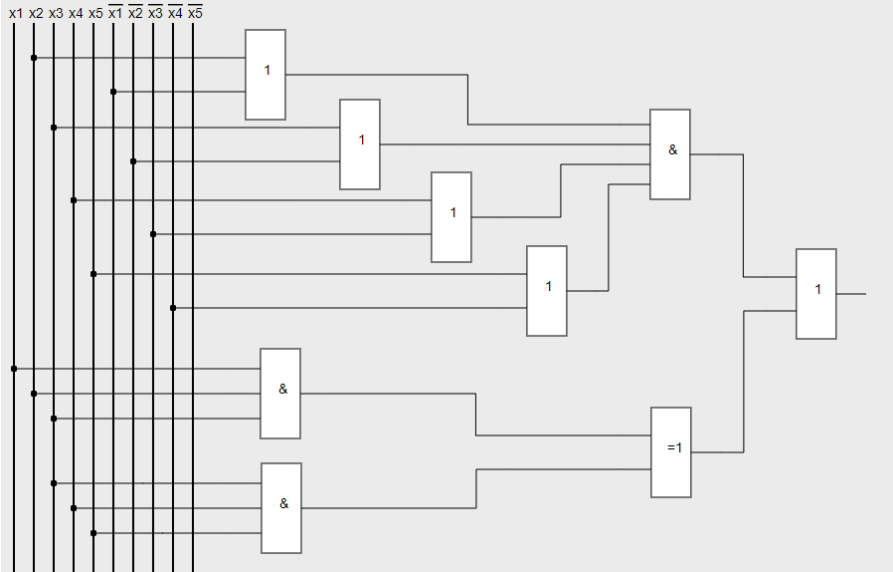
\includegraphics[width=1.0  \linewidth]{images/img}
    \end{figure}

    Сколько существует различных наборов значений переменных x1, x2, x3, x4, x5 таких, что в результате будет получено
    значение 1 (истина)? В ответе укажите число.
    Примечание. На схеме использованы следующие обозначения логических операторов:
    \begin{figure}[h]
        \centering
        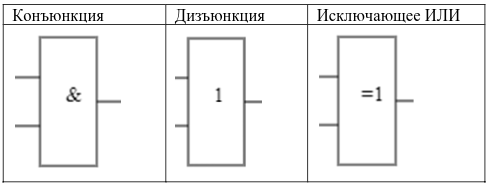
\includegraphics[width=0.6  \linewidth]{images/img_1}
    \end{figure}


\end{document}